\documentclass[11pt,a4paper]{article}

\usepackage{fontspec}
\usepackage[margin=2.2cm]{geometry}
\usepackage{amsmath,amssymb}
\usepackage{booktabs}
\usepackage{float}
\usepackage[font=small,skip=6pt]{caption}
\usepackage{graphicx}
\usepackage{algorithm}
\usepackage[noend]{algpseudocode}
\usepackage{microtype}
\usepackage{enumitem}
\usepackage{xurl}
\usepackage[hidelinks]{hyperref}
\setlist[itemize]{itemsep=2pt, topsep=4pt}

\graphicspath{{../plots/}}
\setlength{\intextsep}{8pt plus 2pt minus 2pt}
\newcommand{\repo}{https://github.com/michaelo-ponteski/evolutionary-computation}
\algnewcommand{\LineComment}[1]{\State \(\triangleright\) #1}

\title{Evolutionary Computation\\[0.3em]\large Lab 1: Greedy heuristics}
\author{Michał Pokładowski \and Oskar Prusinowski}
\date{October 2026}

\begin{document}
\maketitle

\section{Problem description}

We have a set of $n$ nodes. Each node $j$ has a position on a plane and a cost
$c_j$. We have to choose exactly $k = \lceil n/2 \rceil$ nodes and connect them
into a cycle (a Hamiltonian cycle over the chosen nodes). The goal is to make
the length of the cycle plus the costs of the chosen nodes as small as
possible. If a solution is the list of nodes $\pi = (\pi_1, \dots, \pi_k)$, the
objective is
\[
  f(\pi) \;=\; \sum_{i=1}^{k} d_{\pi_i \pi_{i+1}} \;+\; \sum_{i=1}^{k} c_{\pi_i},
  \qquad \pi_{k+1} \equiv \pi_1 ,
\]
where $d_{ij}$ is the Euclidean distance between nodes $i$ and $j$, rounded to
the nearest integer. So we have to decide two things: \emph{which} nodes to
visit and \emph{in what order}.

Both instances, TSPA and TSPB, have 200 nodes, so every solution has 100 nodes.
We compute the distance matrix once, right after reading an instance. The
algorithms use only this matrix and the node costs, not the coordinates.

\section{Implemented algorithms}

As the assignment says, ``nearest'' does not just mean the shortest edge. In
every step the greedy methods choose the option that increases the objective
the least, so they look at the extra distance \emph{and} at the cost of the new
node. If two options are equally good, we take the node with the lower index,
so each greedy method always gives the same result for the same starting node.

When node $j$ is inserted between two neighbouring nodes $a$ and $b$, we add
the edges $a \to j$ and $j \to b$, remove the edge $a \to b$ and pay the cost of
$j$, so the objective grows by
\[
  \Delta(a, j, b) \;=\; d_{aj} + d_{jb} - d_{ab} + c_j .
\]

\begin{algorithm}[H]
\caption{Random solution}
\begin{algorithmic}[1]
\State $P \gets$ random permutation of $V$
\State \Return the first $k$ nodes of $P$
\end{algorithmic}
\end{algorithm}

\begin{algorithm}[H]
\caption{Nearest neighbour, adding nodes only at the end of the path}
\begin{algorithmic}[1]
\Require starting node $s$
\State $P \gets (s)$
\While{$|P| < k$}
  \State $\ell \gets$ last node of $P$
  \State $j^\ast \gets \arg\min_{j \notin P} \; \bigl(d_{\ell j} + c_j\bigr)$
  \State append $j^\ast$ to $P$
\EndWhile
\State \Return $P$ \Comment{the last node connects back to the first}
\end{algorithmic}
\end{algorithm}

\begin{algorithm}[H]
\caption{Nearest neighbour, adding nodes at any position of the path}
\begin{algorithmic}[1]
\Require starting node $s$
\State $P \gets (s)$ \Comment{an open path $(p_1, \dots, p_m)$}
\While{$|P| < k$}
  \ForAll{$j \notin P$}
    \LineComment{cost of each place where $j$ can go}
    \State at the beginning: $\; d_{j p_1} + c_j$
    \State at the end: $\; d_{p_m j} + c_j$
    \State between $p_i$ and $p_{i+1}$, $i = 1, \dots, m-1$: $\; \Delta(p_i, j, p_{i+1})$
  \EndFor
  \State insert the node $j^\ast$ at the cheapest place found for any $j$
\EndWhile
\State \Return $P$ \Comment{the last node connects back to the first}
\end{algorithmic}
\end{algorithm}

\begin{algorithm}[H]
\caption{Greedy cycle}
\begin{algorithmic}[1]
\Require starting node $s$
\State $j' \gets \arg\min_{j \neq s} \; \bigl(d_{sj} + c_j\bigr)$ \Comment{the ``nearest'' node}
\State $C \gets (s, j')$ \Comment{an incomplete cycle $s \to j' \to s$}
\While{$|C| < k$}
  \State $(j^\ast, (a^\ast, b^\ast)) \gets \arg\min_{j \notin C,\; (a,b) \in E(C)} \; \Delta(a, j, b)$
  \Statex \hspace{\algorithmicindent} $E(C)$: all edges of the cycle, also the one from the last node back to the first
  \State insert $j^\ast$ between $a^\ast$ and $b^\ast$
\EndWhile
\State \Return $C$
\end{algorithmic}
\end{algorithm}

Algorithms 3 and 4 differ in one thing. Algorithm 3 builds an open path and
ignores the edge back to the start until the very end. Algorithm 4 keeps a
closed cycle from the beginning, so this edge counts in every step like any
other edge. Both need $O(k^2 n)$ time per solution; Algorithm 2 needs $O(kn)$.

\section{Computational experiment}

We ran each greedy method 200 times, once from every node as the starting
node, and we generated 200 random solutions (with a fixed seed). 200 solutions
take about 0.2\,s for Algorithms 3 and 4 and about 10\,ms for Algorithm 2.
Table~\ref{tab:results} shows the objective values; the best average and the
best minimum for each instance are in bold. Table~\ref{tab:breakdown} shows the
median for the greedy methods and what their average objective is made of.

\begin{table}[H]
\centering
\small
\caption{Objective function values over 200 solutions per method.}
\label{tab:results}
\begin{tabular}{lrrrrrr}
\toprule
 & \multicolumn{3}{c}{TSPA} & \multicolumn{3}{c}{TSPB} \\
\cmidrule(lr){2-4}\cmidrule(lr){5-7}
Method & avg & min & max & avg & min & max \\
\midrule
Random & 261\,928 & 236\,759 & 289\,659 & 205\,907 & 174\,617 & 233\,796 \\
NN (end only) & 87\,477 & 84\,362 & 90\,075 & \textbf{59\,397} & 56\,007 & 63\,166 \\
NN (any position) & 74\,347 & \textbf{72\,328} & 77\,022 & 59\,476 & \textbf{52\,915} & 66\,164 \\
Greedy cycle & \textbf{73\,797} & 72\,590 & 75\,281 & 59\,709 & 53\,016 & 63\,736 \\
\bottomrule
\end{tabular}

\end{table}

\begin{table}[H]
\centering
\small
\caption{Greedy methods: median objective, and average cycle length, node costs and closing edge (part of the length).}
\label{tab:breakdown}
\begin{tabular}{lrrrrrrrr}
\toprule
 & \multicolumn{4}{c}{TSPA} & \multicolumn{4}{c}{TSPB} \\
\cmidrule(lr){2-5}\cmidrule(lr){6-9}
Method & median & length & costs & closing & median & length & costs & closing \\
\midrule
NN (end only) & 87\,594 & 33\,642 & 53\,835 & 1\,452 & 59\,589 & 26\,882 & 32\,515 & 1\,651 \\
NN (any position) & 74\,278 & 23\,072 & 51\,276 & 1\,576 & 60\,254 & 18\,678 & 40\,798 & 2\,031 \\
Greedy cycle & 73\,744 & 22\,309 & 51\,489 & 233 & 59\,167 & 17\,935 & 41\,774 & 194 \\
\bottomrule
\end{tabular}

\end{table}

\clearpage
\section{Best solutions}

Figures~\ref{fig:tspa} and~\ref{fig:tspb} show the best solution of each
method. The colour and the size of a node show its cost; nodes that are not in
the solution are faded. The red dashed line is the edge from the last node of
the list back to the first.

\begin{figure}[H]
\centering
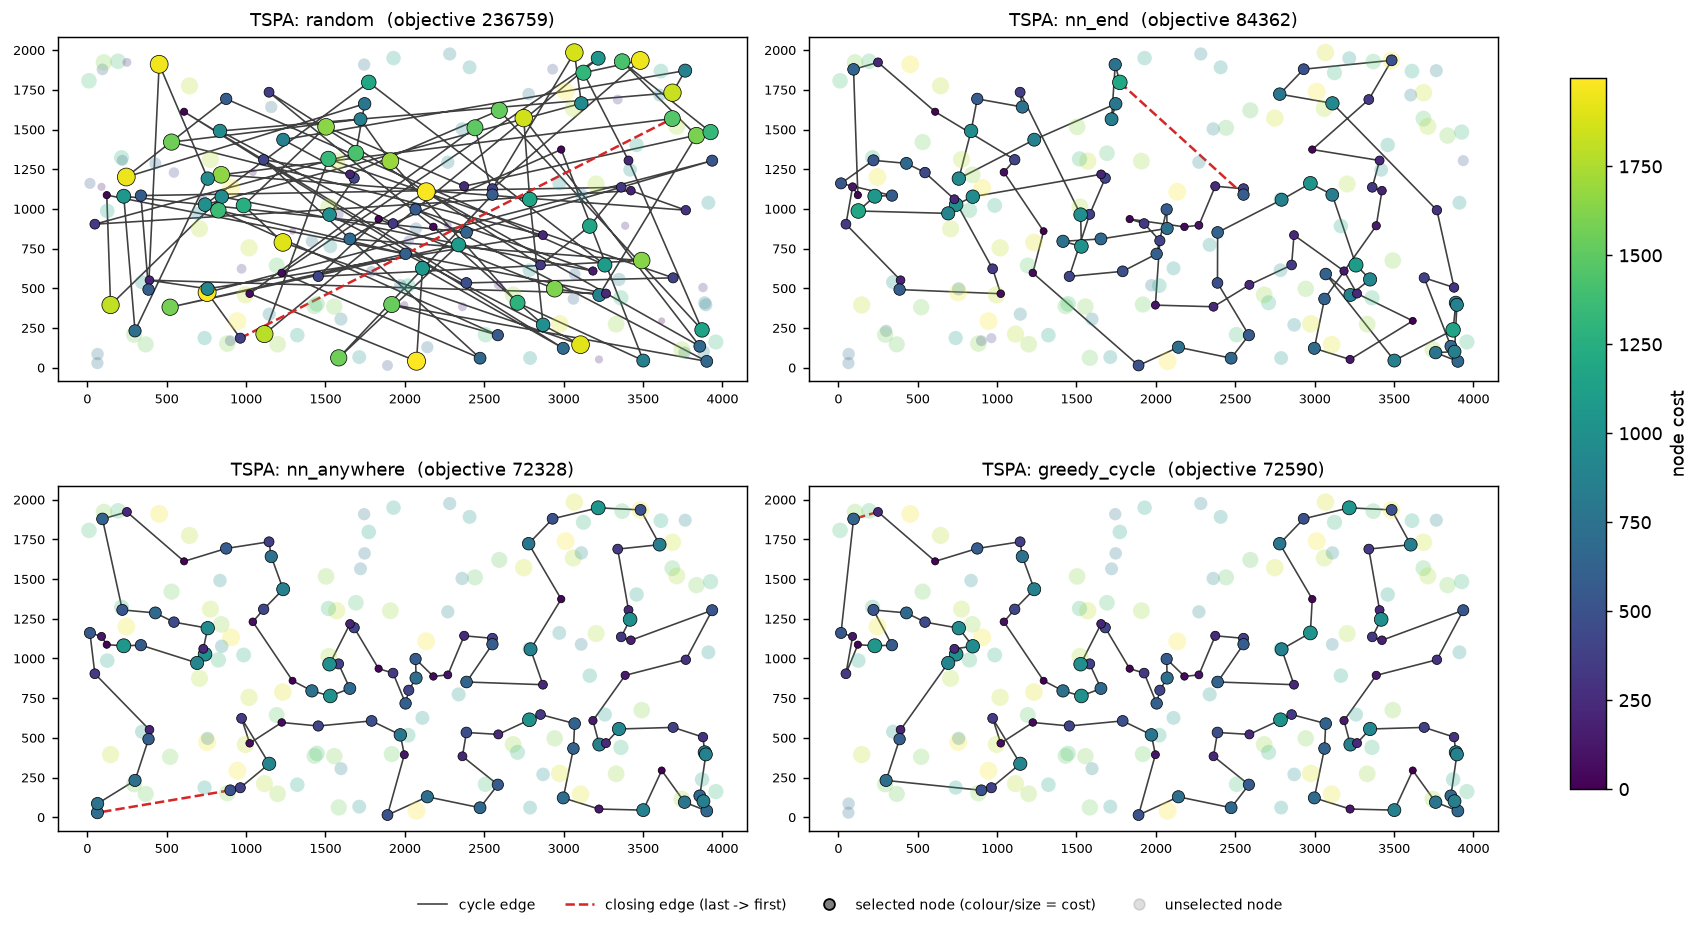
\includegraphics[width=0.93\linewidth]{TSPA.png}
\caption{Best solutions for instance TSPA.}
\label{fig:tspa}
\end{figure}

\begin{figure}[H]
\centering
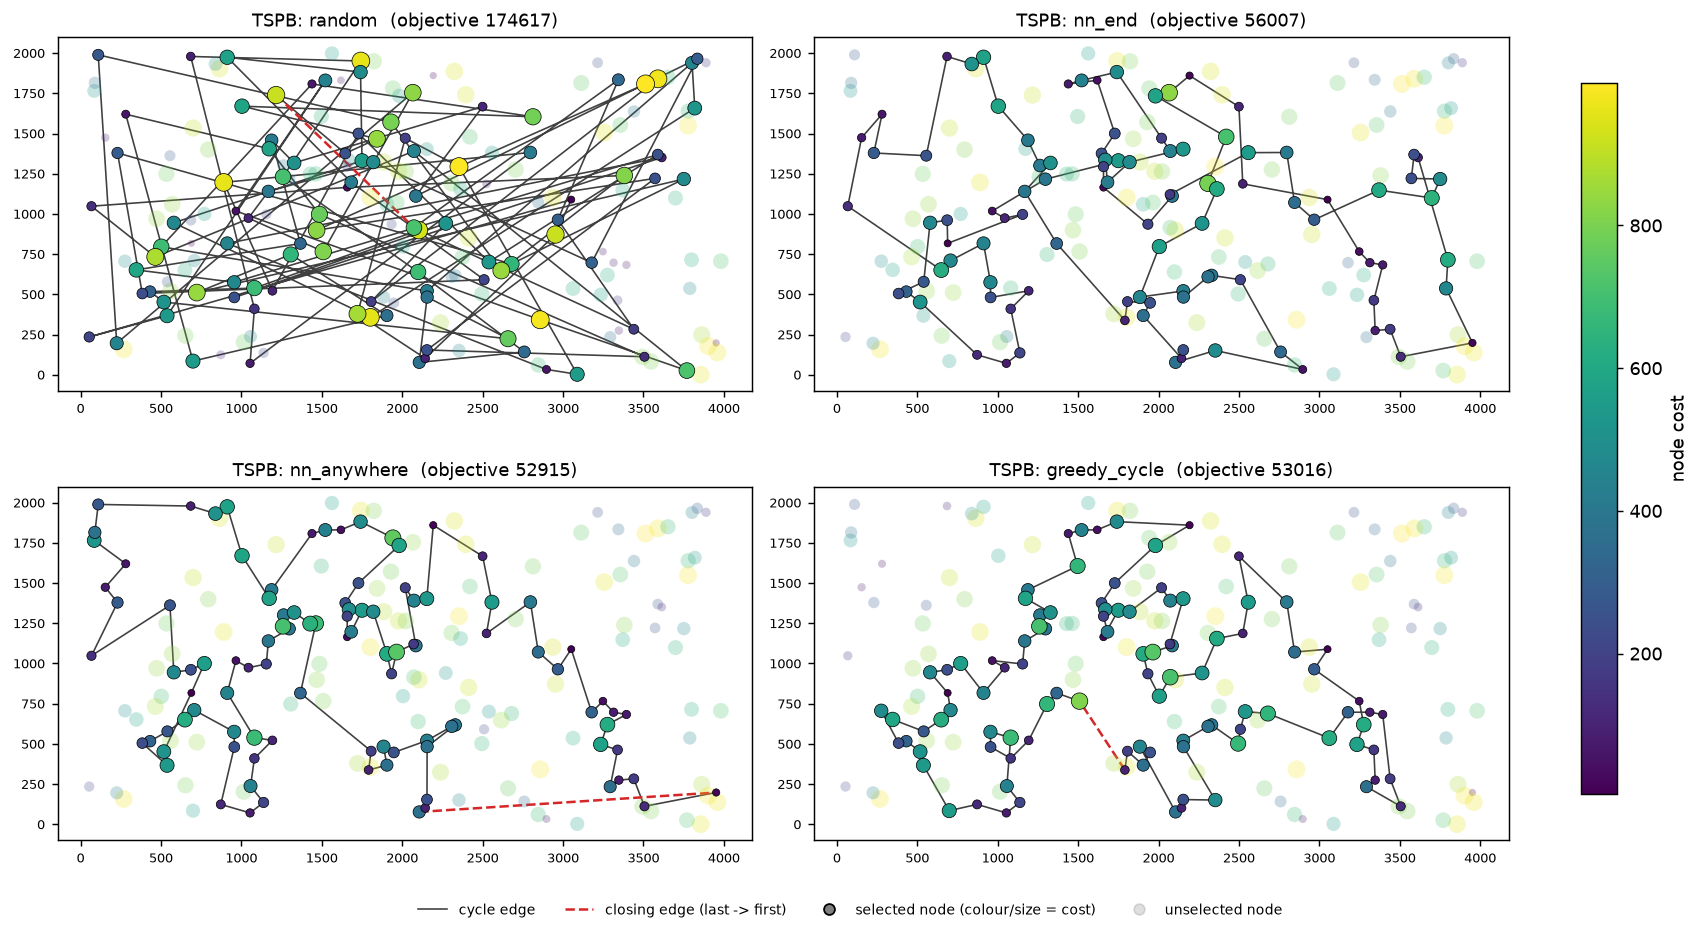
\includegraphics[width=0.93\linewidth]{TSPB.png}
\caption{Best solutions for instance TSPB.}
\label{fig:tspb}
\end{figure}

\subsection*{Best solutions as lists of node indices (starting from 0)}
\paragraph{TSPA, Random}
{\footnotesize\ttfamily\raggedright 46, 44, 47, 50, 168, 133, 112, 167, 91, 43, 5, 83, 184, 197, 9, 79, 24, 1, 75, 34, 51, 76, 192, 141, 163, 166, 196, 130, 84, 80, 182, 41, 118, 187, 15, 54, 22, 99, 120, 140, 148, 158, 121, 78, 52, 106, 90, 188, 63, 89, 97, 161, 174, 66, 139, 190, 65, 64, 164, 144, 38, 86, 55, 4, 16, 156, 105, 191, 162, 18, 33, 21, 19, 6, 42, 0, 67, 87, 117, 185, 74, 153, 109, 194, 138, 177, 157, 176, 81, 3, 49, 127, 126, 100, 69, 11, 131, 147, 125, 2\par}

\paragraph{TSPA, NN (end only)}
{\footnotesize\ttfamily\raggedright 54, 9, 33, 36, 177, 67, 144, 53, 135, 58, 134, 176, 174, 106, 89, 107, 57, 182, 151, 93, 50, 3, 1, 164, 178, 29, 136, 186, 184, 47, 159, 130, 153, 78, 88, 193, 170, 146, 75, 64, 150, 42, 113, 43, 85, 142, 8, 131, 84, 158, 192, 181, 114, 141, 180, 132, 76, 80, 48, 31, 63, 149, 168, 97, 127, 187, 30, 123, 152, 108, 60, 116, 49, 11, 119, 160, 83, 90, 51, 16, 35, 87, 45, 140, 52, 179, 185, 28, 102, 156, 157, 71, 91, 38, 100, 4, 112, 139, 115, 5\par}

\paragraph{TSPA, NN (any position)}
{\footnotesize\ttfamily\raggedright 104, 129, 69, 127, 97, 168, 116, 149, 63, 11, 49, 160, 83, 123, 100, 152, 108, 60, 31, 48, 80, 91, 157, 71, 4, 76, 132, 180, 28, 102, 185, 35, 156, 51, 16, 67, 144, 140, 53, 179, 52, 177, 36, 33, 9, 54, 131, 174, 8, 164, 186, 136, 163, 29, 101, 178, 1, 169, 3, 50, 147, 47, 93, 106, 42, 89, 113, 130, 159, 146, 170, 153, 193, 78, 88, 107, 64, 57, 182, 151, 150, 176, 72, 134, 84, 58, 158, 192, 181, 114, 135, 73, 45, 87, 141, 187, 30, 189, 2, 171\par}

\paragraph{TSPA, Greedy cycle}
{\footnotesize\ttfamily\raggedright 31, 116, 149, 168, 63, 11, 49, 60, 108, 152, 100, 90, 123, 83, 160, 97, 127, 69, 171, 2, 189, 30, 187, 141, 87, 45, 73, 135, 114, 181, 192, 158, 58, 84, 134, 72, 176, 150, 151, 182, 57, 64, 107, 88, 78, 193, 153, 170, 146, 159, 130, 113, 89, 42, 106, 93, 47, 147, 50, 3, 169, 1, 178, 101, 29, 163, 136, 186, 164, 142, 8, 174, 131, 54, 9, 33, 36, 177, 52, 179, 53, 140, 144, 67, 16, 51, 156, 35, 185, 102, 28, 180, 132, 76, 4, 71, 157, 91, 80, 48\par}

\paragraph{TSPB, Random}
{\footnotesize\ttfamily\raggedright 111, 70, 192, 14, 22, 141, 29, 197, 163, 181, 82, 99, 25, 176, 16, 116, 60, 134, 104, 161, 40, 120, 66, 196, 155, 103, 64, 130, 183, 57, 3, 94, 80, 117, 38, 140, 49, 32, 174, 37, 166, 119, 41, 69, 65, 102, 46, 93, 186, 154, 198, 36, 1, 54, 106, 87, 107, 72, 0, 17, 171, 97, 114, 71, 27, 59, 165, 199, 4, 10, 179, 2, 124, 191, 149, 62, 51, 33, 113, 148, 84, 145, 132, 67, 160, 42, 48, 8, 177, 101, 61, 81, 152, 19, 121, 77, 50, 92, 133, 195\par}

\paragraph{TSPB, NN (end only)}
{\footnotesize\ttfamily\raggedright 32, 89, 57, 76, 54, 127, 129, 90, 153, 20, 14, 2, 110, 118, 56, 114, 196, 10, 148, 143, 78, 192, 162, 104, 185, 184, 3, 151, 69, 172, 133, 120, 96, 121, 198, 48, 72, 46, 86, 117, 160, 136, 8, 21, 154, 140, 47, 170, 125, 177, 6, 132, 29, 197, 175, 134, 45, 60, 40, 71, 155, 97, 115, 180, 65, 28, 149, 145, 158, 116, 147, 42, 50, 130, 30, 183, 38, 64, 85, 59, 167, 51, 87, 179, 82, 88, 171, 99, 67, 24, 34, 181, 152, 73, 98, 27, 135, 75, 79, 156\par}

\paragraph{TSPB, NN (any position)}
{\footnotesize\ttfamily\raggedright 110, 2, 14, 20, 74, 153, 182, 52, 90, 129, 127, 80, 54, 192, 162, 104, 76, 185, 57, 89, 86, 46, 72, 3, 184, 173, 151, 122, 117, 8, 160, 69, 172, 136, 133, 120, 156, 43, 48, 96, 198, 121, 130, 191, 50, 42, 147, 116, 37, 146, 13, 149, 28, 145, 65, 158, 177, 125, 26, 170, 197, 36, 132, 29, 6, 180, 115, 155, 71, 175, 134, 45, 157, 60, 40, 141, 97, 154, 140, 47, 38, 21, 176, 30, 183, 189, 168, 64, 59, 85, 51, 73, 167, 152, 34, 24, 181, 179, 87, 82\par}

\paragraph{TSPB, Greedy cycle}
{\footnotesize\ttfamily\raggedright 49, 64, 33, 40, 60, 71, 155, 141, 157, 45, 134, 175, 62, 36, 197, 29, 132, 178, 103, 6, 180, 115, 170, 177, 125, 26, 97, 140, 154, 47, 38, 21, 176, 30, 183, 191, 130, 63, 121, 198, 96, 48, 89, 156, 120, 133, 136, 172, 160, 69, 8, 117, 72, 46, 86, 184, 3, 173, 122, 151, 98, 111, 27, 135, 76, 185, 57, 104, 162, 54, 192, 127, 52, 182, 153, 20, 74, 2, 14, 90, 129, 80, 150, 84, 66, 67, 31, 24, 34, 152, 181, 88, 179, 87, 82, 73, 167, 51, 59, 85\par}


\subsection*{Verification with the solution checker}

We checked all best solutions with the solution checker spreadsheet. We pasted
each list of nodes into the checker, recalculated it and compared its result
with ours (Table~\ref{tab:checker}). All values are the same. We also checked
every solution from the experiment: each one has exactly $k$ different nodes.

\begin{table}[H]
\centering
\small
\caption{Best solutions: our objective value and the value from the checker.}
\label{tab:checker}
\begin{tabular}{lrrrr}
\toprule
 & \multicolumn{2}{c}{TSPA} & \multicolumn{2}{c}{TSPB} \\
\cmidrule(lr){2-3}\cmidrule(lr){4-5}
Method & reported & checker & reported & checker \\
\midrule
Random & 236759 & 236759 & 174617 & 174617 \\
NN (end only) & 84362 & 84362 & 56007 & 56007 \\
NN (any position) & 72328 & 72328 & 52915 & 52915 \\
Greedy cycle & 72590 & 72590 & 53016 & 53016 \\
\bottomrule
\end{tabular}

\end{table}

\section{Source code}

The code is available at \url{\repo/tree/lab1}. It is written in Rust. Code
that later labs will also use (reading instances, distance matrix, objective
function, heuristics) is in \texttt{common/}, the experiment for this lab is in
\texttt{lab1/}, and the Python scripts for the plots and the checker are in
\texttt{scripts/}.

\section{Conclusions}

\begin{itemize}
  \item All greedy methods are much better than random solutions. The average
        drops from about 262\,000 to 74\,000-87\,000 on TSPA and from about
        206\,000 to about 59\,500 on TSPB. A big part of this comes from
        choosing cheap nodes: in the best greedy solutions on TSPA a chosen
        node costs about 510 on average, while the average over all nodes is
        971.
  \item On TSPA, inserting nodes anywhere helps a lot: both insertion methods
        are about 15\,\% better on average than adding nodes only at the end.
        Greedy cycle has the best average and the best worst case, and nearest
        neighbour (any position) found the best single solution, but on
        average they differ by less than 1\,\%.
  \item On TSPB the averages of the three greedy methods are almost the same
        (59\,397-59\,709), but for different reasons (Table~\ref{tab:breakdown}).
        Nearest neighbour (end only) makes 44-50\,\% longer cycles (26\,882
        vs.\ 17\,935-18\,678), but it chooses much cheaper nodes (32\,515
        vs.\ 40\,798-41\,774). On this instance the two effects almost cancel
        out. We think the reason is simple geometry: to add a far, cheap node
        at the end of a path we pay its distance once, but to insert it into
        the cycle we pay about twice as much, because we have to go there and
        come back. So the insertion methods prefer more expensive nodes that
        are close. On TSPA the node costs of the three methods are similar
        (51\,276-53\,835), so the shorter cycles win.
  \item On TSPB the order by average is not reliable. By median, greedy cycle
        is the best (59\,167) and nearest neighbour (any position) is the worst
        (60\,254). Nearest neighbour (any position) also has the widest range
        of results (52\,915 to 66\,164): a few very good solutions, including
        the best one of all methods, pull its average down, while a few weaker
        solutions pull up the average of greedy cycle.
  \item The edge back to the start explains much of this range. Nearest
        neighbour (any position) ignores this edge while building the path, so
        the two ends of the path can end up far apart. On average this edge is
        2\,031 long on TSPB and 1\,576 on TSPA, and in its best TSPB solution
        it is the longest edge of the cycle (1\,850). In greedy cycle it is a
        normal edge (194 and 233 on average), because in every step it can be
        split like any other edge.
  \item Node costs are 56-70\,\% of the objective of the best greedy solutions
        (for example 51\,020 of 72\,590 for the best greedy cycle on TSPA), so
        choosing the right nodes matters at least as much as their order. The
        greedy methods never change a node once it is chosen, so methods that
        can swap chosen and unchosen nodes could improve these solutions a lot.
\end{itemize}

\end{document}
